\documentclass[11pt]{article}

\usepackage[margin=1in]{geometry}
\usepackage{parskip}
\usepackage{amsmath,amssymb,amsthm}
\usepackage{tikz}
\usetikzlibrary{arrows.meta}
\tikzset{lbl/.style={draw=none, fill=none, minimum size=0pt,
  inner sep=1pt, font=\scriptsize}}

\newtheorem{definition}{Definition}
\newtheorem{theorem}{Theorem}

\title{Max-Flow Min-Cut\footnote{can't take credit, but it's sure catchy}}
\author{Daniel Mortensen and Florance Lapierre}
\date{\today}

\begin{document}
\maketitle
\tableofcontents
\newpage

% =====================================================================
\section{Introduction and Example}
% =====================================================================

Many problems reduce to pushing as much material as possible
through a network of limited-capacity links.  Consider the
following directed graph, where each edge has a maximum capacity:

\begin{center}
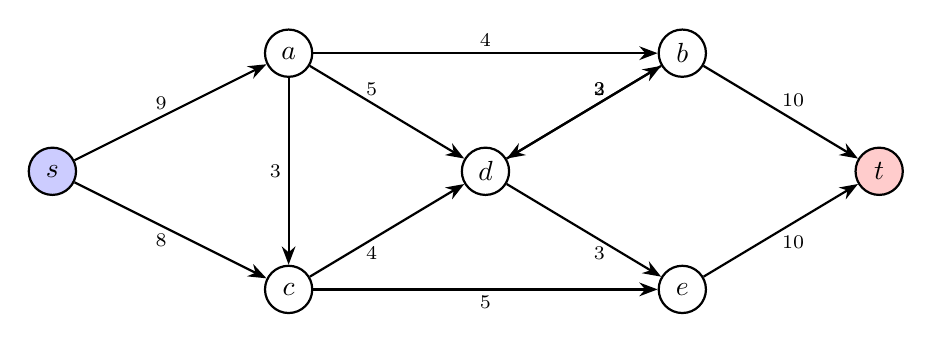
\begin{tikzpicture}[every node/.style={circle, draw, minimum size=6mm,
  inner sep=0pt}, >=Stealth, thick]
  \node[fill=blue!20] (s) at (-2, 0) {$s$};
  \node (a) at (1, 1.5)  {$a$};
  \node (c) at (1, -1.5) {$c$};
  \node (d) at (3.5, 0)  {$d$};
  \node (b) at (6, 1.5)  {$b$};
  \node (e) at (6, -1.5) {$e$};
  \node[fill=red!20] (t) at (8.5, 0) {$t$};
  % edges with capacity labels
  \draw[->] (s) -- node[lbl, above left]  {9} (a);
  \draw[->] (s) -- node[lbl, below left]  {8} (c);
  \draw[->] (a) -- node[lbl, above]       {4} (b);
  \draw[->] (a) -- node[lbl, left]        {3} (c);
  \draw[->] (a) -- node[lbl, above, pos=0.4] {5} (d);
  \draw[->] (c) -- node[lbl, below, pos=0.4] {4} (d);
  \draw[->] (c) -- node[lbl, below]       {5} (e);
  \draw[->] (d) -- node[lbl, above, pos=0.6] {3} (b);
  \draw[->] (d) -- node[lbl, below, pos=0.6] {3} (e);
  \draw[->] (b) -- node[lbl, above, pos=0.4] {2} (d);
  \draw[->] (b) -- node[lbl, above right] {10} (t);
  \draw[->] (e) -- node[lbl, below right] {10} (t);
\end{tikzpicture}
\end{center}

We want to send flow from the \textbf{source} $s$ to the
\textbf{sink} $t$.  Each edge can carry flow up to its capacity,
and at every intermediate node, flow in must equal flow out.  The
network has a rich structure: the node $d$ sits at the centre,
the edges $b \to d$ and $d \to b$ form a cycle, and the
cross-connections $a \to c$, $a \to d$, $c \to d$ create multiple
overlapping routes from $s$ to $t$.  Different paths have
different bottlenecks.

The central question is: \emph{what is the maximum total flow
from $s$ to $t$, and where is the bottleneck?}  We will develop
the tools to answer this in Sections~2--4, then return to this
network for a complete worked example in Section~4.

\subsection{Definitions}

\begin{definition}[Network]
A \textbf{network} is a directed graph $G = (V, E)$ without multiple arcs that contains a
non-negative capacity function $c : E \to \mathbb{R}_{\ge 0}$.
\end{definition}

\begin{definition}[Flow network]
When a \textbf{network} contains a \textbf{source}, denoted $s$, and a \textbf{sink}, denoted $t$ \footnote{...because $t$ totally makes you think sink...}, then $(G, c, s, t)$ is said to be a \textbf{flow network}.
\end{definition}

\begin{definition}[Flow]
A \textbf{flow} is a function $f : E \to \mathbb{R}_{\ge 0}$
satisfying:
\begin{enumerate}
  \item \textbf{Capacity}: $0 \le f(u,v) \le c(u,v)$ for all
        $(u,v) \in E$.
  \item \textbf{Conservation}: for every
        $v \in V \setminus \{s,t\}$,
        \[
          \sum_{u:(u,v)\in E} f(u,v)
          = \sum_{w:(v,w)\in E} f(v,w).
        \]
\end{enumerate}
\end{definition}

\begin{definition}[$s$-$t$ cut]
An \textbf{$s$-$t$ cut} $(S, T)$ is a partition $V = S \cup T$
with $s \in S$ and $t \in T$.  Its \textbf{capacity} is
\[
  c(S,T) = \sum_{\substack{u \in S,\, v \in T \\ (u,v) \in E}}
           c(u,v).
\]
\end{definition}

\section{Min-Cut/Max-Flow}

The goal is to show that the maximum flow equals the minimum
cut.  The argument has three parts:

\begin{enumerate}
  \item \textbf{Cuts bound flows} (Section~2.1)---we revisit
        why every cut is a bipartite bottleneck in general graphs.
  \item \textbf{Ford--Fulkerson algorithm} (Section~3)---we
        construct an algorithm that repeatedly pushes flow along
        augmenting paths until none remain.
  \item \textbf{The theorem} (Section~4)---when the algorithm
        terminates, the final residual graph reveals a cut whose
        capacity equals the flow value, proving
        $\max |f| = \min c(S,T)$.
\end{enumerate}

\subsection{Cuts Bound Flows}

\textbf{Claim.} For any flow $f$ and any $s$-$t$ cut $(S,T)$,
$|f| \le c(S,T)$.

\begin{proof}
Let $(S,T)$ be any $s$-$t$ cut and $f$ any flow.

\medskip\noindent
\textbf{Step 1.}  Every unit of flow from $s$ to $t$ must cross
the cut at least once, because $s \in S$ and $t \in T$.  Some
flow may also cross back from $T$ to $S$.  Therefore the value
of the flow equals the \emph{net} flow across the cut:
\[
  |f|
  = \underbrace{\sum_{\substack{u \in S \\ v \in T}} f(u,v)
    }_{\text{flow from } S \text{ to } T}
  \;-\; \underbrace{\sum_{\substack{u \in T \\ v \in S}} f(u,v)
    }_{\text{flow from } T \text{ to } S}.
\]

\medskip\noindent
\textbf{Step 2.}  The second sum is non-negative (all flows are
$\ge 0$), so dropping it can only increase the right-hand side:
\[
  |f| \;\le\; \sum_{\substack{u \in S \\ v \in T}} f(u,v).
\]

\medskip\noindent
\textbf{Step 3.}  Each term $f(u,v)$ satisfies the capacity
constraint $f(u,v) \le c(u,v)$, so:
\[
  \sum_{\substack{u \in S \\ v \in T}} f(u,v)
  \;\le\; \sum_{\substack{u \in S \\ v \in T}} c(u,v)
  \;=\; c(S,T).
\]
\medskip\noindent
and hence, $\;|f| \le c(S,T)$.
\end{proof}

The key insight is knowing that finding a flow $f$ and a cut $(S,T)$
with $|f| = c(S,T)$ actually guarantees that $f$ is the maximum flow, and $(S,T)$ is a minimum cut.
The max-flow min-cut theorem
(Section~5) guarantees that such a pair always exists.

\subsection{Are they Equal?}
\subsubsection{Matchings}

A \textbf{matching} $M \subseteq E$ is a set of edges with no
shared endpoints.  A vertex is \textbf{matched} if it belongs to
some edge in $M$; otherwise it is \textbf{free}.  A
\textbf{maximum matching} maximises $|M|$.  A \textbf{perfect
matching} matches every vertex ($|M| = |U| = |V|$).

\subsubsection{Alternating and Augmenting Paths}

Given a matching $M$, an \textbf{alternating path} alternates
between edges in $M$ and edges not in $M$.  An
\textbf{augmenting path} is an alternating path whose two
endpoints are both free.

If an augmenting path exists, flipping every edge along it
(matched $\leftrightarrow$ unmatched) yields a matching of size
$|M| + 1$.

\begin{theorem}[Berge, 1957]
A matching $M$ is maximum if and only if there is no augmenting
path with respect to $M$.
\end{theorem}

Consider the bipartite graph with $U = \{u_1, u_2, u_3, u_4\}$,
$V = \{v_1, v_2, v_3, v_4\}$ and edges:

\begin{center}
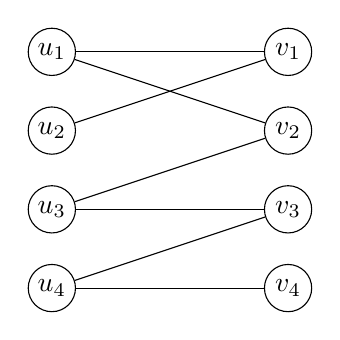
\begin{tikzpicture}[every node/.style={circle, draw, minimum size=6mm,
  inner sep=0pt}, >=Stealth]
  \foreach \i in {1,...,4} {
    \node (u\i) at (0, -\i) {$u_\i$};
    \node (v\i) at (3, -\i) {$v_\i$};
  }
  \draw (u1)--(v1); \draw (u1)--(v2);
  \draw (u2)--(v1);
  \draw (u3)--(v2); \draw (u3)--(v3);
  \draw (u4)--(v3); \draw (u4)--(v4);
\end{tikzpicture}
\end{center}

Note that $u_2$ has only one neighbour ($v_1$), so any perfect
matching must assign $u_2 \to v_1$.  The algorithm does not know
this in advance.

\paragraph{Step 1.}
$M = \emptyset$.  Search from $u_1$ (free): find $v_1$ (free).
Augmenting path $u_1\text{--}v_1$.  Augment.

\begin{center}
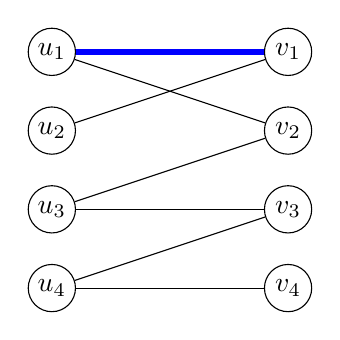
\begin{tikzpicture}[every node/.style={circle, draw, minimum size=6mm,
  inner sep=0pt}, >=Stealth]
  \foreach \i in {1,...,4} {
    \node (u\i) at (0, -\i) {$u_\i$};
    \node (v\i) at (3, -\i) {$v_\i$};
  }
  \draw[line width=2pt, blue] (u1)--(v1);
  \draw (u1)--(v2);
  \draw (u2)--(v1);
  \draw (u3)--(v2); \draw (u3)--(v3);
  \draw (u4)--(v3); \draw (u4)--(v4);
\end{tikzpicture}
\end{center}

$M = \{(u_1, v_1)\}$, $|M| = 1$.

\paragraph{Step 2.}
Search from $u_3$ (free): find $v_2$ (free).
Augmenting path $u_3\text{--}v_2$.  Augment.

\begin{center}
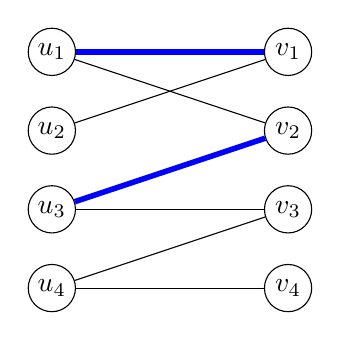
\begin{tikzpicture}[every node/.style={circle, draw, minimum size=6mm,
  inner sep=0pt}, >=Stealth]
  \foreach \i in {1,...,4} {
    \node (u\i) at (0, -\i) {$u_\i$};
    \node (v\i) at (3, -\i) {$v_\i$};
  }
  \draw[line width=2pt, blue] (u1)--(v1);
  \draw (u1)--(v2);
  \draw (u2)--(v1);
  \draw[line width=2pt, blue] (u3)--(v2);
  \draw (u3)--(v3);
  \draw (u4)--(v3); \draw (u4)--(v4);
\end{tikzpicture}
\end{center}

$M = \{(u_1, v_1),\, (u_3, v_2)\}$, $|M| = 2$.

\paragraph{Step 3.}
Search from $u_4$ (free): find $v_3$ (free).
Augmenting path $u_4\text{--}v_3$.  Augment.

\begin{center}
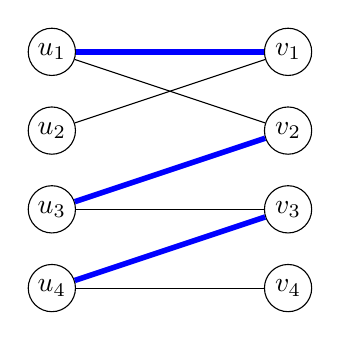
\begin{tikzpicture}[every node/.style={circle, draw, minimum size=6mm,
  inner sep=0pt}, >=Stealth]
  \foreach \i in {1,...,4} {
    \node (u\i) at (0, -\i) {$u_\i$};
    \node (v\i) at (3, -\i) {$v_\i$};
  }
  \draw[line width=2pt, blue] (u1)--(v1);
  \draw (u1)--(v2);
  \draw (u2)--(v1);
  \draw[line width=2pt, blue] (u3)--(v2);
  \draw (u3)--(v3);
  \draw[line width=2pt, blue] (u4)--(v3);
  \draw (u4)--(v4);
\end{tikzpicture}
\end{center}

$M = \{(u_1, v_1),\, (u_3, v_2),\, (u_4, v_3)\}$, $|M| = 3$.

\paragraph{Step 4.}
The only free vertex in $U$ is $u_2$.  Its sole neighbour is
$v_1$, which is matched to $u_1$.  No free vertex is directly
reachable, so BFS must follow alternating edges through the
matching:

\[
  \underset{\text{free}}{u_2}
  \xrightarrow{\;\text{unmatched}\;}
  v_1
  \xrightarrow{\;\text{matched}\;}
  u_1
  \xrightarrow{\;\text{unmatched}\;}
  v_2
  \xrightarrow{\;\text{matched}\;}
  u_3
  \xrightarrow{\;\text{unmatched}\;}
  v_3
  \xrightarrow{\;\text{matched}\;}
  u_4
  \xrightarrow{\;\text{unmatched}\;}
  \underset{\text{free}}{v_4}
\]

This is an augmenting path of length~7 (four unmatched edges,
three matched edges).  Flipping every edge along the path yields:

\begin{center}
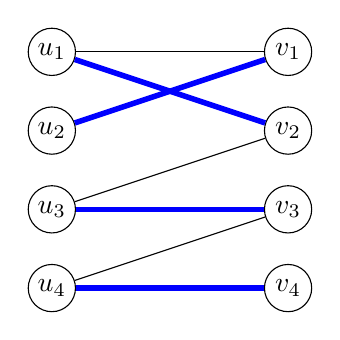
\begin{tikzpicture}[every node/.style={circle, draw, minimum size=6mm,
  inner sep=0pt}, >=Stealth]
  \foreach \i in {1,...,4} {
    \node (u\i) at (0, -\i) {$u_\i$};
    \node (v\i) at (3, -\i) {$v_\i$};
  }
  \draw (u1)--(v1);
  \draw[line width=2pt, blue] (u1)--(v2);
  \draw[line width=2pt, blue] (u2)--(v1);
  \draw (u3)--(v2);
  \draw[line width=2pt, blue] (u3)--(v3);
  \draw (u4)--(v3);
  \draw[line width=2pt, blue] (u4)--(v4);
\end{tikzpicture}
\end{center}

$M = \{(u_2, v_1),\, (u_1, v_2),\, (u_3, v_3),\, (u_4, v_4)\}$,
$|M| = 4$.  This is a perfect matching.

\paragraph{Step 5.}
No free vertices remain.  No augmenting path exists.  By Berge's
theorem, $M$ is a maximum matching.

\medskip
The key observation is Step~4: the algorithm rerouted three
existing matched edges through a single augmenting path.  The
``cascade'' $v_1 \to u_1 \to v_2 \to u_3 \to v_3 \to u_4$
displaced every previous assignment to make room for $u_2$.
Without this ability to undo prior choices, a greedy algorithm
would be stuck at $|M| = 3$.

% =====================================================================
\subsubsection{Beyond Bipartite}
% =====================================================================

Flow and cuts apply not only to bipartite networks but to
arbitrary directed graphs.  The reason is that every cut in a
general graph \emph{already is} a bipartite bottleneck.

To illustrate, consider the following flow network built from the
bipartite graph in Section~1 by adding a source $s$ and sink $t$
with unit-capacity edges:

\begin{center}
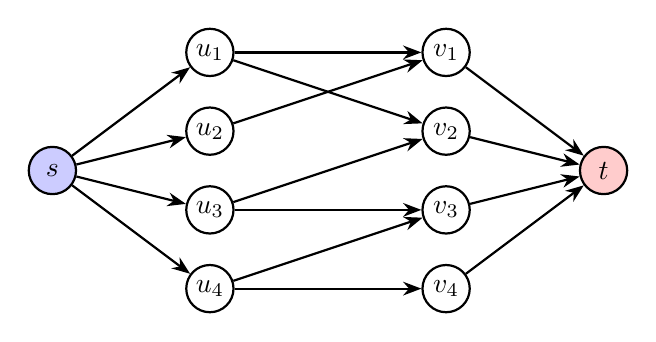
\begin{tikzpicture}[every node/.style={circle, draw, minimum size=6mm,
  inner sep=0pt}, >=Stealth, thick]
  \node[fill=blue!20] (s) at (-2, -2.5) {$s$};
  \node[fill=red!20]  (t) at (5, -2.5)  {$t$};
  \foreach \i in {1,...,4} {
    \node (u\i) at (0, -\i) {$u_\i$};
    \node (v\i) at (3, -\i) {$v_\i$};
  }
  \foreach \i in {1,...,4} {
    \draw[->] (s)--(u\i);
    \draw[->] (v\i)--(t);
  }
  \draw[->] (u1)--(v1); \draw[->] (u1)--(v2);
  \draw[->] (u2)--(v1);
  \draw[->] (u3)--(v2); \draw[->] (u3)--(v3);
  \draw[->] (u4)--(v3); \draw[->] (u4)--(v4);
\end{tikzpicture}
\end{center}


\subsection{Hall's Theorem}

\begin{theorem}[Hall, 1935]
A bipartite graph $G = (U \cup V, E)$ has a matching saturating
every vertex in $U$ iff $|N(S)| \ge |S|$ for all
$S \subseteq U$.
\end{theorem}

Hall's condition is equivalent to every $s$-$t$ cut having
capacity at least $|U|$ in the corresponding flow network.

\subsection{Every Cut Is a Bipartite Interface}

Take any $s$-$t$ cut $(S, T)$ in a directed graph.  The edges
crossing from $S$ to $T$ form a bipartite structure: each has
one endpoint in $S$ and one in $T$.  Every unit of flow from $s$
to $t$ must cross this interface.

Consider the cut $S = \{s, u_1, u_2\}$,
$T = \{u_3, u_4, v_1, v_2, v_3, v_4, t\}$ in our flow network:

\begin{center}
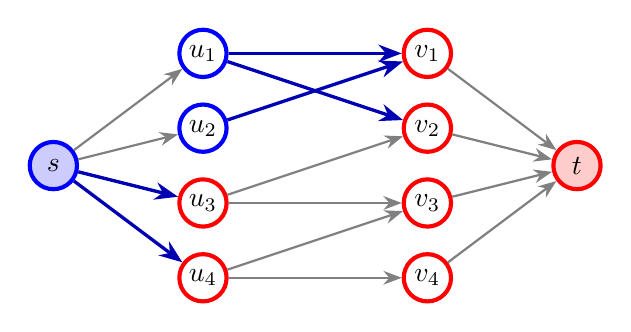
\begin{tikzpicture}[every node/.style={circle, draw, minimum size=6mm,
  inner sep=0pt}, >=Stealth, thick, scale=0.95,
  snode/.style={draw=blue, line width=1.5pt},
  tnode/.style={draw=red, line width=1.5pt}]
  \node[snode, fill=blue!20] (s) at (-2, -2.5) {$s$};
  \node[tnode, fill=red!20]  (t) at (5, -2.5)  {$t$};
  \node[snode] (u1) at (0, -1) {$u_1$};
  \node[snode] (u2) at (0, -2) {$u_2$};
  \node[tnode] (u3) at (0, -3) {$u_3$};
  \node[tnode] (u4) at (0, -4) {$u_4$};
  \foreach \i in {1,...,4} {
    \node[tnode] (v\i) at (3, -\i) {$v_\i$};
  }
  % Internal S edges (gray)
  \draw[->, gray] (s)--(u1);
  \draw[->, gray] (s)--(u2);
  % Cut edges (bold) -- from S to T
  \draw[->, very thick, blue!70!black] (s)--(u3);
  \draw[->, very thick, blue!70!black] (s)--(u4);
  \draw[->, very thick, blue!70!black] (u1)--(v1);
  \draw[->, very thick, blue!70!black] (u1)--(v2);
  \draw[->, very thick, blue!70!black] (u2)--(v1);
  % Edges entirely in T (gray)
  \draw[->, gray] (u3)--(v2); \draw[->, gray] (u3)--(v3);
  \draw[->, gray] (u4)--(v3); \draw[->, gray] (u4)--(v4);
  \foreach \i in {1,...,4} { \draw[->, gray] (v\i)--(t); }
\end{tikzpicture}
\end{center}

The five bold edges cross from
\textcolor{blue}{$S = \{s, u_1, u_2\}$} to
\textcolor{red}{$T = \{u_3, u_4, v_1, v_2, v_3, v_4, t\}$}
(capacity~5); the gray edges are internal plumbing.  No matter
what happens inside $S$ or $T$, flow from $s$ to $t$ cannot
exceed~5 through this cut.

From the perspective of the cut, the internal structure on each
side is irrelevant---only the crossing matters:

\begin{center}
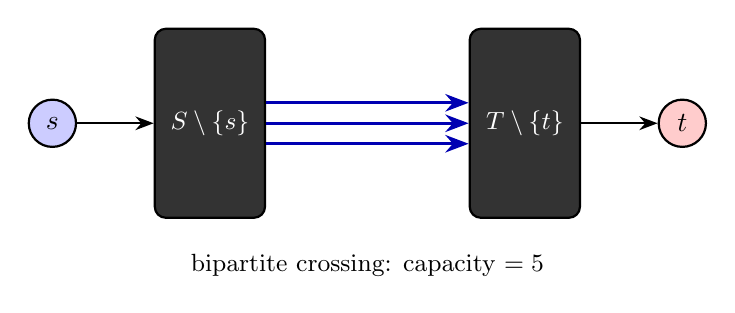
\begin{tikzpicture}[>=Stealth, thick]
  % Source
  \node[circle, draw, fill=blue!20, minimum size=6mm, inner sep=0pt]
    (s) at (0,0) {$s$};
  % S-side black box
  \node[draw, fill=black!80, rounded corners, minimum width=1.4cm,
    minimum height=2.4cm, text=white, font=\small, align=center]
    (sbox) at (2,0) {$S \setminus \{s\}$};
  % T-side black box
  \node[draw, fill=black!80, rounded corners, minimum width=1.4cm,
    minimum height=2.4cm, text=white, font=\small, align=center]
    (tbox) at (6,0) {$T \setminus \{t\}$};
  % Sink
  \node[circle, draw, fill=red!20, minimum size=6mm, inner sep=0pt]
    (t) at (8,0) {$t$};
  % s to S-box
  \draw[->] (s) -- (sbox);
  % Cut edges (bipartite crossing)
  \draw[->, very thick, blue!70!black] (sbox.20) -- (tbox.160);
  \draw[->, very thick, blue!70!black] (sbox.0) -- (tbox.180);
  \draw[->, very thick, blue!70!black] (sbox.-20) -- (tbox.200);
  % T-box to t
  \draw[->] (tbox) -- (t);
  % Label
  \node[draw=none, font=\small] at (4, -1.8)
    {bipartite crossing: capacity $= 5$};
\end{tikzpicture}
\end{center}

The black boxes hide arbitrarily complex subgraphs.  All that
determines the throughput bound is the capacity of the edges
between them.

% =====================================================================
\section{The Ford--Fulkerson Algorithm}
% =====================================================================

\subsection{From Bipartite Matching to Network Flow}

A bipartite matching problem is a network flow problem in
disguise.  We convert the bipartite graph from Section~1 into a
flow network by adding a source $s$ with capacity-1 edges to
every $u \in U$, a sink $t$ with capacity-1 edges from every
$v \in V$, and directing the original edges from $U$ to $V$ with
capacity~1.  All capacities are~1.  (This is the same network
introduced in Section~3.)

An integer maximum flow in this network corresponds exactly to a
maximum matching: each unit of flow along
$s \to u_i \to v_j \to t$ represents the matched edge
$(u_i, v_j)$.

\subsection{Residual Graphs and Augmenting Paths}

Given flow $f$, the \textbf{residual graph} $G_f = (V, E_f)$
contains a \textbf{forward edge} $(u,v)$ with capacity
$c_f(u,v) = c(u,v) - f(u,v)$ whenever this is positive, and a
\textbf{backward edge} $(v,u)$ with capacity $c_f(v,u) = f(u,v)$
whenever $f(u,v) > 0$.  An \textbf{augmenting path} is any
$s \to t$ path in $G_f$.  Backward edges allow the algorithm to
undo previously pushed flow---the same mechanism as augmenting
paths in matching.

\subsection{Ford--Fulkerson on the Bipartite Network}

We now trace the Ford--Fulkerson algorithm on the bipartite flow
network.  At each step we show the residual graph, find an
augmenting $s \to t$ path, and push one unit of flow.  Edges
labelled with their residual capacity; forward edges are solid,
backward edges are dashed.

\paragraph{Iteration 1.}
All flows are zero.  The residual graph equals the original
network.  BFS from $s$ finds the path
$s \to u_1 \to v_1 \to t$ with bottleneck
$\delta = 1$.  Push 1 unit.

Flow: $f(s,u_1) = f(u_1,v_1) = f(v_1,t) = 1$.  Total $|f| = 1$.

\begin{center}
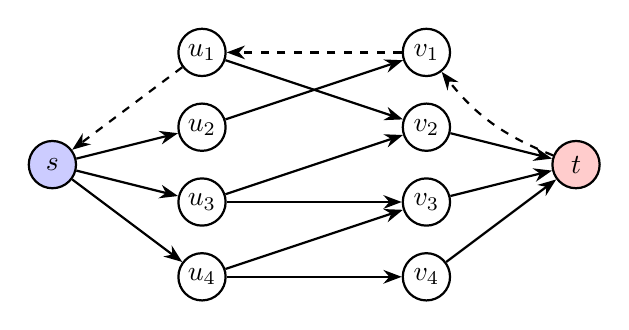
\begin{tikzpicture}[every node/.style={circle, draw, minimum size=6mm,
  inner sep=0pt}, >=Stealth, thick, scale=0.95]
  \node[fill=blue!20] (s) at (-2, -2.5) {$s$};
  \node[fill=red!20]  (t) at (5, -2.5)  {$t$};
  \foreach \i in {1,...,4} {
    \node (u\i) at (0, -\i) {$u_\i$};
    \node (v\i) at (3, -\i) {$v_\i$};
  }
  % s -> U: u1 saturated (backward only), rest forward
  \draw[->, dashed] (u1)--(s);
  \draw[->] (s)--(u2); \draw[->] (s)--(u3); \draw[->] (s)--(u4);
  % V -> t: v1 saturated (backward only), rest forward
  \draw[->, dashed] (t) to[bend left=15] (v1);
  \draw[->] (v2)--(t); \draw[->] (v3)--(t); \draw[->] (v4)--(t);
  % U -> V edges
  \draw[->, dashed] (v1)--(u1);  % backward: f(u1,v1)=1
  \draw[->] (u1)--(v2);          % forward: still unused
  \draw[->] (u2)--(v1);          % forward: still unused
  \draw[->] (u3)--(v2); \draw[->] (u3)--(v3);
  \draw[->] (u4)--(v3); \draw[->] (u4)--(v4);
\end{tikzpicture}
\end{center}

Note the backward edges $u_1 \dashleftarrow v_1$,
$s \dashleftarrow u_1$, and $v_1 \dashleftarrow t$: these allow
future iterations to undo this flow.

\paragraph{Iteration 2.}
BFS from $s$ finds $s \to u_3 \to v_2 \to t$.  Push 1 unit.

Flow: additionally $f(s,u_3) = f(u_3,v_2) = f(v_2,t) = 1$.
Total $|f| = 2$.

\paragraph{Iteration 3.}
BFS from $s$ finds $s \to u_4 \to v_3 \to t$.  Push 1 unit.

Flow: additionally $f(s,u_4) = f(u_4,v_3) = f(v_3,t) = 1$.
Total $|f| = 3$.

The residual graph after three iterations:

\begin{center}
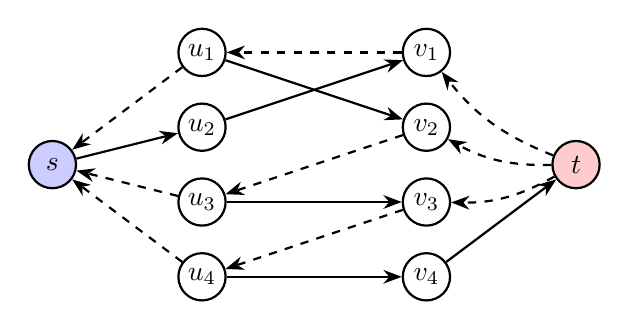
\begin{tikzpicture}[every node/.style={circle, draw, minimum size=6mm,
  inner sep=0pt}, >=Stealth, thick, scale=0.95]
  \node[fill=blue!20] (s) at (-2, -2.5) {$s$};
  \node[fill=red!20]  (t) at (5, -2.5)  {$t$};
  \foreach \i in {1,...,4} {
    \node (u\i) at (0, -\i) {$u_\i$};
    \node (v\i) at (3, -\i) {$v_\i$};
  }
  % s -> U: u1,u3,u4 saturated; u2 open
  \draw[->, dashed] (u1)--(s);
  \draw[->] (s)--(u2);
  \draw[->, dashed] (u3)--(s);
  \draw[->, dashed] (u4)--(s);
  % V -> t: v1,v2,v3 saturated; v4 open
  \draw[->, dashed] (t) to[bend left=15] (v1);
  \draw[->, dashed] (t) to[bend left=15] (v2);
  \draw[->, dashed] (t) to[bend left=15] (v3);
  \draw[->] (v4)--(t);
  % U -> V: saturated edges become backward; unused stay forward
  \draw[->, dashed] (v1)--(u1);   % backward
  \draw[->] (u1)--(v2);           % forward (unused)
  \draw[->] (u2)--(v1);           % forward (unused)
  \draw[->, dashed] (v2)--(u3);   % backward
  \draw[->] (u3)--(v3);           % forward (unused)
  \draw[->, dashed] (v3)--(u4);   % backward
  \draw[->] (u4)--(v4);           % forward (unused)
\end{tikzpicture}
\end{center}

\paragraph{Iteration 4.}
BFS from $s$.  The only forward edge from $s$ is $s \to u_2$.
From $u_2$, the only forward edge is $u_2 \to v_1$.  But
$v_1 \to t$ is saturated (only the backward edge $t \to v_1$
exists).  So BFS must use the backward edge $v_1 \to u_1$
(undoing the flow $u_1 \to v_1$), then the forward edge
$u_1 \to v_2$, then backward $v_2 \to u_3$, then forward
$u_3 \to v_3$, then backward $v_3 \to u_4$, then forward
$u_4 \to v_4$, then forward $v_4 \to t$.

The augmenting path in the residual graph:
\[
  s \to u_2 \to v_1
  \dashrightarrow u_1 \to v_2
  \dashrightarrow u_3 \to v_3
  \dashrightarrow u_4 \to v_4 \to t
\]

\noindent
where $\to$ denotes a forward edge and $\dashrightarrow$ a
backward edge (undoing existing flow).

Bottleneck $\delta = 1$ (all residual capacities are~1).  Push
1 unit along this path.  For each forward edge, increase flow by
1; for each backward edge, \emph{decrease} flow by 1 on the
reverse arc:

\medskip
\begin{center}
\renewcommand{\arraystretch}{1.2}
\begin{tabular}{lll}
  \textbf{Edge in path} & \textbf{Type} & \textbf{Update} \\
  \hline
  $s \to u_2$    & forward  & $f(s,u_2) : 0 \to 1$ \\
  $u_2 \to v_1$  & forward  & $f(u_2,v_1) : 0 \to 1$ \\
  $v_1 \to u_1$  & backward & $f(u_1,v_1) : 1 \to 0$ \\
  $u_1 \to v_2$  & forward  & $f(u_1,v_2) : 0 \to 1$ \\
  $v_2 \to u_3$  & backward & $f(u_3,v_2) : 1 \to 0$ \\
  $u_3 \to v_3$  & forward  & $f(u_3,v_3) : 0 \to 1$ \\
  $v_3 \to u_4$  & backward & $f(u_4,v_3) : 1 \to 0$ \\
  $u_4 \to v_4$  & forward  & $f(u_4,v_4) : 0 \to 1$ \\
  $v_4 \to t$    & forward  & $f(v_4,t) : 0 \to 1$ \\
\end{tabular}
\end{center}

\medskip
Total $|f| = 4$.  The resulting flow (and corresponding matching):

\begin{center}
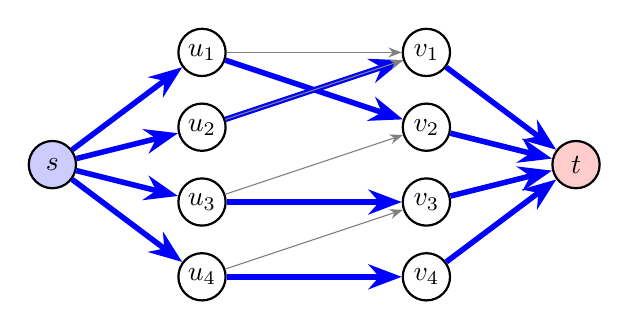
\begin{tikzpicture}[every node/.style={circle, draw, minimum size=6mm,
  inner sep=0pt}, >=Stealth, thick, scale=0.95]
  \node[fill=blue!20] (s) at (-2, -2.5) {$s$};
  \node[fill=red!20]  (t) at (5, -2.5)  {$t$};
  \foreach \i in {1,...,4} {
    \node (u\i) at (0, -\i) {$u_\i$};
    \node (v\i) at (3, -\i) {$v_\i$};
  }
  % flow-carrying edges in blue
  \draw[->, line width=2pt, blue] (s)--(u1);
  \draw[->, line width=2pt, blue] (s)--(u2);
  \draw[->, line width=2pt, blue] (s)--(u3);
  \draw[->, line width=2pt, blue] (s)--(u4);
  \draw[->, line width=2pt, blue] (u2)--(v1);
  \draw[->, line width=2pt, blue] (u1)--(v2);
  \draw[->, line width=2pt, blue] (u3)--(v3);
  \draw[->, line width=2pt, blue] (u4)--(v4);
  \draw[->, line width=2pt, blue] (v1)--(t);
  \draw[->, line width=2pt, blue] (v2)--(t);
  \draw[->, line width=2pt, blue] (v3)--(t);
  \draw[->, line width=2pt, blue] (v4)--(t);
  % non-flow edges (thin gray)
  \draw[->, gray, thin] (u1)--(v1);
  \draw[->, gray, thin] (u2)--(v1);
  \draw[->, gray, thin] (u3)--(v2);
  \draw[->, gray, thin] (u4)--(v3);
\end{tikzpicture}
\end{center}

\paragraph{Iteration 5.}
In the residual graph, all edges from $s$ are saturated (backward
only).  No $s \to t$ path exists.  The algorithm terminates.

The set of vertices reachable from $s$ in the final residual
graph is $S^* = \{s\}$ (no forward edge leaves $s$).  The
minimum cut is $(\{s\}, V \setminus \{s\})$ with capacity~4,
confirming $\max |f| = \min c(S,T) = 4$.

\paragraph{Comparison with Section~1.}
The flow in iteration~4 corresponds exactly to the augmenting
path in Step~4 of the matching algorithm.  The backward edges in
the residual graph play the same role as the matched edges in the
alternating path: they let the algorithm \emph{undo} previous
flow assignments.  Ford--Fulkerson on the flow network is the
augmenting-paths algorithm in disguise.

This connection runs deeper: the minimum cut in the flow network
corresponds to a \emph{minimum vertex cover} in the original
bipartite graph---a smallest set of vertices that touches every
edge.  The fact that max matching always equals min vertex cover
in bipartite graphs is K\"onig's theorem (Section~5.2), and it is
exactly what the max-flow min-cut theorem becomes when applied to
bipartite matching.

\subsection{Max-Flow Algorithm}

\noindent\textbf{Input:} Flow network $(G, c, s, t)$.\\
\textbf{Output:} Maximum flow $f$.

\medskip
\begin{enumerate}
  \item Set $f(u,v) \gets 0$ for all $(u,v) \in E$.
  \item While there exists an augmenting path $P$ in $G_f$:
    \begin{enumerate}
      \item Let $\delta = \min_{(u,v) \in P} c_f(u,v)$.
      \item For each forward edge $(u,v) \in P$, set
            $f(u,v) \gets f(u,v) + \delta$.
      \item For each backward edge $(v,u) \in P$, set
            $f(v,u) \gets f(v,u) - \delta$.
    \end{enumerate}
  \item Return $f$.
\end{enumerate}

\medskip

\subsection{Example: The General Network}

We now return to the general network from Section~1 and trace the
Ford--Fulkerson algorithm (using BFS) from start to finish.
Recall the network:

\begin{center}
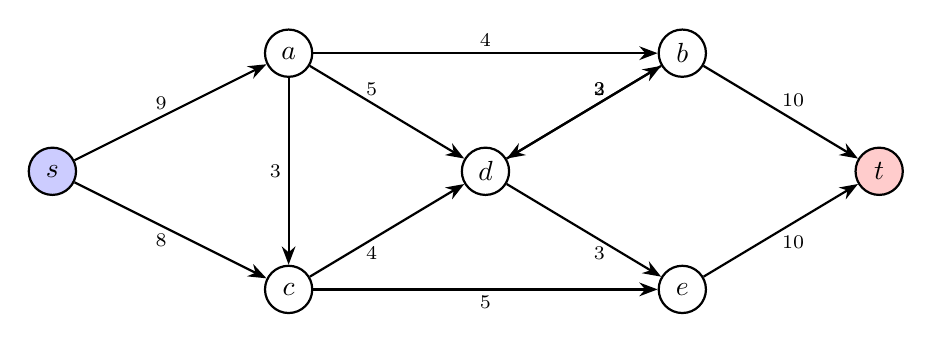
\begin{tikzpicture}[every node/.style={circle, draw, minimum size=6mm,
  inner sep=0pt}, >=Stealth, thick]
  \node[fill=blue!20] (s) at (-2, 0) {$s$};
  \node (a) at (1, 1.5)  {$a$};
  \node (c) at (1, -1.5) {$c$};
  \node (d) at (3.5, 0)  {$d$};
  \node (b) at (6, 1.5)  {$b$};
  \node (e) at (6, -1.5) {$e$};
  \node[fill=red!20] (t) at (8.5, 0) {$t$};
  \draw[->] (s) -- node[lbl, above left]  {9} (a);
  \draw[->] (s) -- node[lbl, below left]  {8} (c);
  \draw[->] (a) -- node[lbl, above]       {4} (b);
  \draw[->] (a) -- node[lbl, left]        {3} (c);
  \draw[->] (a) -- node[lbl, above, pos=0.4] {5} (d);
  \draw[->] (c) -- node[lbl, below, pos=0.4] {4} (d);
  \draw[->] (c) -- node[lbl, below]       {5} (e);
  \draw[->] (d) -- node[lbl, above, pos=0.6] {3} (b);
  \draw[->] (d) -- node[lbl, below, pos=0.6] {3} (e);
  \draw[->] (b) -- node[lbl, above, pos=0.4] {2} (d);
  \draw[->] (b) -- node[lbl, above right] {10} (t);
  \draw[->] (e) -- node[lbl, below right] {10} (t);
\end{tikzpicture}
\end{center}

All flows start at zero.  The residual graph initially equals the
original network.

\paragraph{Iteration 1.}
BFS from $s$ finds the shortest augmenting path
$s \to a \to b \to t$.  Bottleneck:
$\delta = \min(9, 4, 10) = 4$.  Push 4 units.

\medskip
\begin{center}
\renewcommand{\arraystretch}{1.2}
\begin{tabular}{ll}
  \textbf{Edge} & \textbf{Update} \\
  \hline
  $s \to a$ & $f : 0 \to 4$ \\
  $a \to b$ & $f : 0 \to 4$ \\
  $b \to t$ & $f : 0 \to 4$ \\
\end{tabular}
\end{center}

\medskip
Total $|f| = 4$.  The edge $a \to b$ is now saturated.

\paragraph{Iteration 2.}
BFS finds $s \to c \to e \to t$.
Bottleneck: $\delta = \min(8, 5, 10) = 5$.  Push 5 units.

\medskip
\begin{center}
\renewcommand{\arraystretch}{1.2}
\begin{tabular}{ll}
  \textbf{Edge} & \textbf{Update} \\
  \hline
  $s \to c$ & $f : 0 \to 5$ \\
  $c \to e$ & $f : 0 \to 5$ \\
  $e \to t$ & $f : 0 \to 5$ \\
\end{tabular}
\end{center}

\medskip
Total $|f| = 9$.  The edge $c \to e$ is now saturated.

The residual graph after two iterations:

\begin{center}
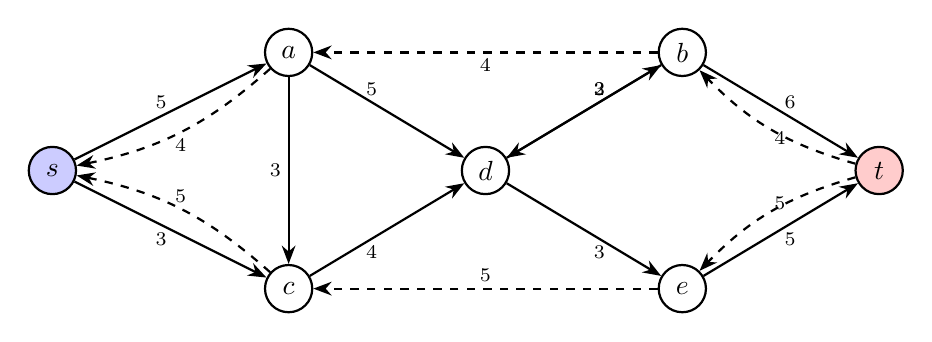
\begin{tikzpicture}[every node/.style={circle, draw, minimum size=6mm,
  inner sep=0pt}, >=Stealth, thick]
  \node[fill=blue!20] (s) at (-2, 0) {$s$};
  \node (a) at (1, 1.5)  {$a$};
  \node (c) at (1, -1.5) {$c$};
  \node (d) at (3.5, 0)  {$d$};
  \node (b) at (6, 1.5)  {$b$};
  \node (e) at (6, -1.5) {$e$};
  \node[fill=red!20] (t) at (8.5, 0) {$t$};
  % Forward edges (with residual capacity)
  \draw[->] (s) -- node[lbl, above left]  {5} (a);
  \draw[->] (s) -- node[lbl, below left]  {3} (c);
  \draw[->] (a) -- node[lbl, left]        {3} (c);
  \draw[->] (a) -- node[lbl, above, pos=0.4] {5} (d);
  \draw[->] (c) -- node[lbl, below, pos=0.4] {4} (d);
  \draw[->] (d) -- node[lbl, above, pos=0.6] {3} (b);
  \draw[->] (d) -- node[lbl, below, pos=0.6] {3} (e);
  \draw[->] (b) -- node[lbl, above, pos=0.4] {2} (d);
  \draw[->] (b) -- node[lbl, above right] {6} (t);
  \draw[->] (e) -- node[lbl, below right] {5} (t);
  % Backward edges (dashed)
  \draw[->, dashed] (a) to[bend left=15]
    node[lbl, below] {4} (s);
  \draw[->, dashed] (b) -- node[lbl, below] {4} (a);
  \draw[->, dashed] (c) to[bend right=15]
    node[lbl, above] {5} (s);
  \draw[->, dashed] (e) -- node[lbl, above] {5} (c);
  \draw[->, dashed] (t) to[bend left=15]
    node[lbl, below right] {4} (b);
  \draw[->, dashed] (t) to[bend right=15]
    node[lbl, above right] {5} (e);
\end{tikzpicture}
\end{center}

The two direct short paths ($s \to a \to b \to t$ and
$s \to c \to e \to t$) have been partially or fully used.
All remaining augmenting paths must route through the central
node~$d$.

\paragraph{Iteration 3.}
BFS finds the length-4 path $s \to a \to d \to b \to t$.
Bottleneck: $\delta = \min(5, 5, 3, 6) = 3$.  Push 3 units.

\medskip
\begin{center}
\renewcommand{\arraystretch}{1.2}
\begin{tabular}{ll}
  \textbf{Edge} & \textbf{Update} \\
  \hline
  $s \to a$ & $f : 4 \to 7$ \\
  $a \to d$ & $f : 0 \to 3$ \\
  $d \to b$ & $f : 0 \to 3$ \\
  $b \to t$ & $f : 4 \to 7$ \\
\end{tabular}
\end{center}

\medskip
Total $|f| = 12$.  The edge $d \to b$ is now saturated; flow
now enters $b$ from two sources ($a$ and~$d$).

\paragraph{Iteration 4.}
With $d \to b$ saturated, BFS finds
$s \to a \to d \to e \to t$.
Bottleneck: $\delta = \min(2, 2, 3, 5) = 2$.  Push 2 units.

\medskip
\begin{center}
\renewcommand{\arraystretch}{1.2}
\begin{tabular}{ll}
  \textbf{Edge} & \textbf{Update} \\
  \hline
  $s \to a$ & $f : 7 \to 9$ \\
  $a \to d$ & $f : 3 \to 5$ \\
  $d \to e$ & $f : 0 \to 2$ \\
  $e \to t$ & $f : 5 \to 7$ \\
\end{tabular}
\end{center}

\medskip
Total $|f| = 14$.  The edges $s \to a$ and $a \to d$ are now
saturated.

\paragraph{Iteration 5.}
With $s \to a$ saturated, the only forward edge from $s$ is
$s \to c$ (residual capacity~3).  BFS explores: from $c$, the
edge $c \to e$ is saturated, so only $c \to d$ (capacity~4) is
available.  From $d$, both $d \to b$ and $d \to e$ have limited
residual capacity.

BFS finds $s \to c \to d \to e \to t$.
Bottleneck: $\delta = \min(3, 4, 1, 3) = 1$.  Push 1 unit.

\medskip
\begin{center}
\renewcommand{\arraystretch}{1.2}
\begin{tabular}{ll}
  \textbf{Edge} & \textbf{Update} \\
  \hline
  $s \to c$ & $f : 5 \to 6$ \\
  $c \to d$ & $f : 0 \to 1$ \\
  $d \to e$ & $f : 2 \to 3$ \\
  $e \to t$ & $f : 7 \to 8$ \\
\end{tabular}
\end{center}

\medskip
Total $|f| = 15$.  The edge $d \to e$ is now saturated.

\paragraph{Termination.}
BFS from $s$: the only forward edge is $s \to c$ (residual
capacity~2).  From $c$, we reach $d$ (via $c \to d$, capacity~3).
From $d$, both $d \to b$ and $d \to e$ are saturated.  The
backward edge from $d$ reaches $a$, but from $a$ all forward
edges are saturated.  No path to $t$ exists.  The algorithm
terminates with maximum flow $|f^*| = 15$.

The final flow on every edge:

\begin{center}
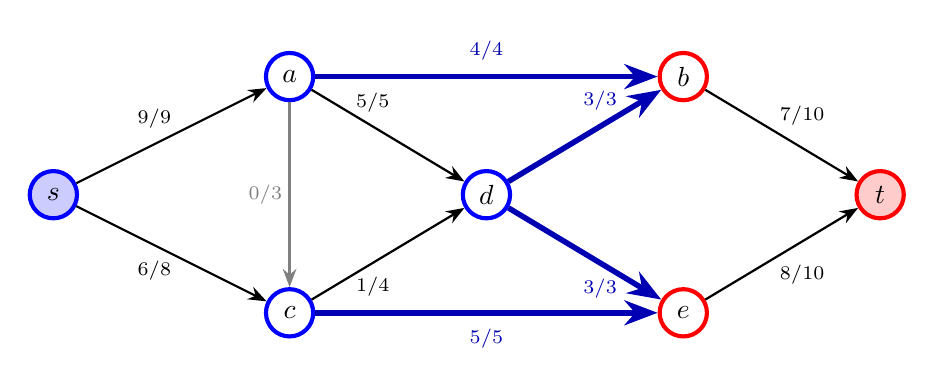
\begin{tikzpicture}[every node/.style={circle, draw, minimum size=6mm,
  inner sep=0pt}, >=Stealth, thick,
  snode/.style={draw=blue, line width=1.5pt},
  tnode/.style={draw=red, line width=1.5pt}]
  \node[snode, fill=blue!20] (s) at (-2, 0) {$s$};
  \node[snode] (a) at (1, 1.5)  {$a$};
  \node[snode] (c) at (1, -1.5) {$c$};
  \node[snode] (d) at (3.5, 0)  {$d$};
  \node[tnode] (b) at (6, 1.5)  {$b$};
  \node[tnode] (e) at (6, -1.5) {$e$};
  \node[tnode, fill=red!20] (t) at (8.5, 0) {$t$};
  % internal S edges (gray)
  \draw[->] (s) -- node[lbl, above left] {$9/9$} (a);
  \draw[->] (s) -- node[lbl, below left] {$6/8$} (c);
  \draw[->, gray] (a) -- node[lbl, left] {$0/3$} (c);
  \draw[->] (a) -- node[lbl, above, pos=0.4] {$5/5$} (d);
  \draw[->] (c) -- node[lbl, below, pos=0.4] {$1/4$} (d);
  % cut edges (blue, bold) -- from S to T
  \draw[->, line width=2pt, blue!70!black] (a) --
    node[lbl, above] {$4/4$} (b);
  \draw[->, line width=2pt, blue!70!black] (c) --
    node[lbl, below] {$5/5$} (e);
  \draw[->, line width=2pt, blue!70!black] (d) --
    node[lbl, above, pos=0.6] {$3/3$} (b);
  \draw[->, line width=2pt, blue!70!black] (d) --
    node[lbl, below, pos=0.6] {$3/3$} (e);
  % internal T edges (gray)
%  \draw[->, gray] (b) -- node[lbl, above, pos=0.4] {$0/2$} (d);
  \draw[->] (b) -- node[lbl, above right] {$7/10$} (t);
  \draw[->] (e) -- node[lbl, below right] {$8/10$} (t);
\end{tikzpicture}
\end{center}

Verify conservation at each node:
\begin{itemize}
  \item $a$: in $= 9$, out $= 4 + 0 + 5 = 9$.
  \item $b$: in $= 4 + 3 = 7$, out $= 0 + 7 = 7$.
  \item $c$: in $= 6 + 0 = 6$, out $= 1 + 5 = 6$.
  \item $d$: in $= 5 + 1 = 6$, out $= 3 + 3 = 6$.
  \item $e$: in $= 5 + 3 = 8$, out $= 8$.
\end{itemize}

\paragraph{The minimum cut.}
The vertices reachable from $s$ in the final residual graph are
$S^* = \{s, a, c, d\}$: from $s$ we reach $c$ (residual
capacity~2 on $s \to c$); from $c$ we reach $d$ (via $c \to d$,
residual~3); from $d$ we reach $a$ via the backward edge
(since $a \to d$ carries flow~5).  But from none of these can we
reach $b$, $e$, or $t$---every crossing edge is saturated.

The minimum cut is
$(\{s, a, c, d\},\; \{b, e, t\})$ with capacity
\[
  c(a, b) + c(d, b) + c(c, e) + c(d, e)
  = 4 + 3 + 5 + 3 = 15 = |f^*|.
\]

This confirms the max-flow min-cut theorem: the maximum flow
equals the capacity of the tightest bottleneck.  The bottleneck
is not at $s$ (total outgoing capacity~17) or at $t$ (total
incoming capacity~20), but at the internal boundary between
$\{s, a, c, d\}$ and $\{b, e, t\}$---the four edges that cross
from the source side to the sink side are all fully saturated.

% =====================================================================
\section{The Max-Flow Min-Cut Theorem}
% =====================================================================

\subsection{Statement}

\begin{theorem}[Ford--Fulkerson, 1956]
\label{thm:mfmc}
In any flow network $(G, c, s, t)$,
\[
  \max_f |f| = \min_{(S,T)} c(S,T).
\]
\end{theorem}

The following are equivalent: (i)~$f$ is a maximum flow;
(ii)~there is no augmenting path in the residual graph $G_f$;
(iii)~$|f| = c(S,T)$ for some cut $(S,T)$.

\subsection{Proof}

In Section~1 we showed that $|f| \le c(S,T)$ for every flow $f$
and every cut $(S,T)$.  It remains to show that equality is
achieved.

\textbf{Claim.} There exist $f^*$ and $(S^*,T^*)$ with
$|f^*| = c(S^*,T^*)$.

\begin{proof}
Run Ford--Fulkerson until no augmenting path exists; call the
resulting flow $f^*$.  Define
\[
  S^* = \{v \in V : v \text{ reachable from } s \text{ in }
        G_{f^*}\}, \qquad T^* = V \setminus S^*.
\]
Since $t \notin S^*$, this is a valid cut.  For every edge
$(u,v)$ with $u \in S^*$, $v \in T^*$ we have
$f^*(u,v) = c(u,v)$---otherwise $v$ would be reachable via a
forward edge.  For every edge $(v,u)$ with $v \in T^*$,
$u \in S^*$ we have $f^*(v,u) = 0$---otherwise $v$ would be
reachable via a backward edge.  Therefore
\[
  |f^*|
  = \sum_{\substack{u \in S^*,\, v \in T^*}} f^*(u,v)
  - \sum_{\substack{v \in T^*,\, u \in S^*}} f^*(v,u)
  = c(S^*,T^*) - 0
  = c(S^*,T^*).
\]
Since every cut bounds every flow, $f^*$ is a maximum flow and
$(S^*,T^*)$ is a minimum cut.
\end{proof}

% =====================================================================
\section{Related Results}
% =====================================================================

The max-flow min-cut theorem is the cornerstone of a family of
results in combinatorics.

\subsection{Menger's Theorem}

\begin{theorem}[Menger, 1927]
The maximum number of vertex-disjoint $s$-$t$ paths equals the
minimum number of vertices (other than $s,t$) whose removal
disconnects $s$ from $t$.
\end{theorem}

The edge-disjoint version---max edge-disjoint paths equals min
edge cut---is a direct corollary of max-flow min-cut with unit
capacities.

\subsection{K\"onig--Egerv\'ary Theorem}

\begin{theorem}[K\"onig, 1931; Egerv\'ary, 1931]
In a bipartite graph, the size of a maximum matching equals the
size of a minimum vertex cover.
\end{theorem}

A vertex cover is a set of vertices touching every edge.  The
minimum vertex cover corresponds to a minimum cut in the flow
network.

\subsection{Birkhoff--von Neumann Theorem}

\begin{theorem}[Birkhoff, 1946; von Neumann, 1953]
Every doubly stochastic matrix is a convex combination of
permutation matrices.
\end{theorem}

A \textbf{doubly stochastic matrix} is a square matrix with
non-negative entries whose rows each sum to~1 and whose columns
each sum to~1.  A \textbf{permutation matrix} is the special case
where every entry is 0 or 1---it picks exactly one entry per row
and one per column (i.e.\ a perfect matching).

The theorem says that every doubly stochastic matrix can be
written as a weighted average of permutation matrices.  In the
language of matchings: if we allow fractional matchings (assigning
a weight between 0 and 1 to each edge, so that every vertex's
weights sum to at most~1), then the optimal fractional matching
has the same value as the optimal integer matching.  Relaxing the
problem to allow fractions does not help---the integer solution
is already optimal.

\end{document}
